% Options for packages loaded elsewhere
\PassOptionsToPackage{unicode}{hyperref}
\PassOptionsToPackage{hyphens}{url}
%
\documentclass[
  11pt,
  letterpaper,
  DIV=11,
  numbers=noendperiod,
  twoside]{scrartcl}

\usepackage{amsmath,amssymb}
\usepackage{setspace}
\usepackage{iftex}
\ifPDFTeX
  \usepackage[T1]{fontenc}
  \usepackage[utf8]{inputenc}
  \usepackage{textcomp} % provide euro and other symbols
\else % if luatex or xetex
  \usepackage{unicode-math}
  \defaultfontfeatures{Scale=MatchLowercase}
  \defaultfontfeatures[\rmfamily]{Ligatures=TeX,Scale=1}
\fi
\usepackage{lmodern}
\ifPDFTeX\else  
    % xetex/luatex font selection
    \setmainfont[ItalicFont=EB Garamond Italic,BoldFont=EB Garamond
Bold]{EB Garamond Math}
    \setsansfont[]{EB Garamond}
  \setmathfont[]{Garamond-Math}
\fi
% Use upquote if available, for straight quotes in verbatim environments
\IfFileExists{upquote.sty}{\usepackage{upquote}}{}
\IfFileExists{microtype.sty}{% use microtype if available
  \usepackage[]{microtype}
  \UseMicrotypeSet[protrusion]{basicmath} % disable protrusion for tt fonts
}{}
\usepackage{xcolor}
\usepackage[left=1.1in, right=1in, top=0.8in, bottom=0.8in,
paperheight=9.5in, paperwidth=7in, includemp=TRUE, marginparwidth=0in,
marginparsep=0in]{geometry}
\setlength{\emergencystretch}{3em} % prevent overfull lines
\setcounter{secnumdepth}{3}
% Make \paragraph and \subparagraph free-standing
\makeatletter
\ifx\paragraph\undefined\else
  \let\oldparagraph\paragraph
  \renewcommand{\paragraph}{
    \@ifstar
      \xxxParagraphStar
      \xxxParagraphNoStar
  }
  \newcommand{\xxxParagraphStar}[1]{\oldparagraph*{#1}\mbox{}}
  \newcommand{\xxxParagraphNoStar}[1]{\oldparagraph{#1}\mbox{}}
\fi
\ifx\subparagraph\undefined\else
  \let\oldsubparagraph\subparagraph
  \renewcommand{\subparagraph}{
    \@ifstar
      \xxxSubParagraphStar
      \xxxSubParagraphNoStar
  }
  \newcommand{\xxxSubParagraphStar}[1]{\oldsubparagraph*{#1}\mbox{}}
  \newcommand{\xxxSubParagraphNoStar}[1]{\oldsubparagraph{#1}\mbox{}}
\fi
\makeatother


\providecommand{\tightlist}{%
  \setlength{\itemsep}{0pt}\setlength{\parskip}{0pt}}\usepackage{longtable,booktabs,array}
\usepackage{calc} % for calculating minipage widths
% Correct order of tables after \paragraph or \subparagraph
\usepackage{etoolbox}
\makeatletter
\patchcmd\longtable{\par}{\if@noskipsec\mbox{}\fi\par}{}{}
\makeatother
% Allow footnotes in longtable head/foot
\IfFileExists{footnotehyper.sty}{\usepackage{footnotehyper}}{\usepackage{footnote}}
\makesavenoteenv{longtable}
\usepackage{graphicx}
\makeatletter
\newsavebox\pandoc@box
\newcommand*\pandocbounded[1]{% scales image to fit in text height/width
  \sbox\pandoc@box{#1}%
  \Gscale@div\@tempa{\textheight}{\dimexpr\ht\pandoc@box+\dp\pandoc@box\relax}%
  \Gscale@div\@tempb{\linewidth}{\wd\pandoc@box}%
  \ifdim\@tempb\p@<\@tempa\p@\let\@tempa\@tempb\fi% select the smaller of both
  \ifdim\@tempa\p@<\p@\scalebox{\@tempa}{\usebox\pandoc@box}%
  \else\usebox{\pandoc@box}%
  \fi%
}
% Set default figure placement to htbp
\def\fps@figure{htbp}
\makeatother
% definitions for citeproc citations
\NewDocumentCommand\citeproctext{}{}
\NewDocumentCommand\citeproc{mm}{%
  \begingroup\def\citeproctext{#2}\cite{#1}\endgroup}
\makeatletter
 % allow citations to break across lines
 \let\@cite@ofmt\@firstofone
 % avoid brackets around text for \cite:
 \def\@biblabel#1{}
 \def\@cite#1#2{{#1\if@tempswa , #2\fi}}
\makeatother
\newlength{\cslhangindent}
\setlength{\cslhangindent}{1.5em}
\newlength{\csllabelwidth}
\setlength{\csllabelwidth}{3em}
\newenvironment{CSLReferences}[2] % #1 hanging-indent, #2 entry-spacing
 {\begin{list}{}{%
  \setlength{\itemindent}{0pt}
  \setlength{\leftmargin}{0pt}
  \setlength{\parsep}{0pt}
  % turn on hanging indent if param 1 is 1
  \ifodd #1
   \setlength{\leftmargin}{\cslhangindent}
   \setlength{\itemindent}{-1\cslhangindent}
  \fi
  % set entry spacing
  \setlength{\itemsep}{#2\baselineskip}}}
 {\end{list}}
\usepackage{calc}
\newcommand{\CSLBlock}[1]{\hfill\break\parbox[t]{\linewidth}{\strut\ignorespaces#1\strut}}
\newcommand{\CSLLeftMargin}[1]{\parbox[t]{\csllabelwidth}{\strut#1\strut}}
\newcommand{\CSLRightInline}[1]{\parbox[t]{\linewidth - \csllabelwidth}{\strut#1\strut}}
\newcommand{\CSLIndent}[1]{\hspace{\cslhangindent}#1}

\usepackage{booktabs}
\usepackage{longtable}
\usepackage{array}
\usepackage{multirow}
\usepackage{wrapfig}
\usepackage{float}
\usepackage{colortbl}
\usepackage{pdflscape}
\usepackage{tabu}
\usepackage{threeparttable}
\usepackage{threeparttablex}
\usepackage[normalem]{ulem}
\usepackage{makecell}
\usepackage{xcolor}
\setlength\heavyrulewidth{0ex}
\setlength\lightrulewidth{0ex}
\usepackage[automark]{scrlayer-scrpage}
\clearpairofpagestyles
\cehead{
  Brian Weatherson
  }
\cohead{
  Mixing Expert Opinion
  }
\ohead{\bfseries \pagemark}
\cfoot{}
\makeatletter
\newcommand*\NoIndentAfterEnv[1]{%
  \AfterEndEnvironment{#1}{\par\@afterindentfalse\@afterheading}}
\makeatother
\NoIndentAfterEnv{itemize}
\NoIndentAfterEnv{enumerate}
\NoIndentAfterEnv{description}
\NoIndentAfterEnv{quote}
\NoIndentAfterEnv{equation}
\NoIndentAfterEnv{longtable}
\NoIndentAfterEnv{abstract}
\renewenvironment{abstract}
 {\vspace{-1.25cm}
 \quotation\small\noindent\emph{Abstract}:}
 {\endquotation}
\newfontfamily\tfont{EB Garamond}
\addtokomafont{disposition}{\rmfamily}
\addtokomafont{title}{\normalfont\itshape}
\let\footnoterule\relax
\KOMAoption{captions}{tableheading}
\makeatletter
\@ifpackageloaded{caption}{}{\usepackage{caption}}
\AtBeginDocument{%
\ifdefined\contentsname
  \renewcommand*\contentsname{Table of contents}
\else
  \newcommand\contentsname{Table of contents}
\fi
\ifdefined\listfigurename
  \renewcommand*\listfigurename{List of Figures}
\else
  \newcommand\listfigurename{List of Figures}
\fi
\ifdefined\listtablename
  \renewcommand*\listtablename{List of Tables}
\else
  \newcommand\listtablename{List of Tables}
\fi
\ifdefined\figurename
  \renewcommand*\figurename{Figure}
\else
  \newcommand\figurename{Figure}
\fi
\ifdefined\tablename
  \renewcommand*\tablename{Table}
\else
  \newcommand\tablename{Table}
\fi
}
\@ifpackageloaded{float}{}{\usepackage{float}}
\floatstyle{ruled}
\@ifundefined{c@chapter}{\newfloat{codelisting}{h}{lop}}{\newfloat{codelisting}{h}{lop}[chapter]}
\floatname{codelisting}{Listing}
\newcommand*\listoflistings{\listof{codelisting}{List of Listings}}
\makeatother
\makeatletter
\makeatother
\makeatletter
\@ifpackageloaded{caption}{}{\usepackage{caption}}
\@ifpackageloaded{subcaption}{}{\usepackage{subcaption}}
\makeatother

\usepackage{bookmark}

\IfFileExists{xurl.sty}{\usepackage{xurl}}{} % add URL line breaks if available
\urlstyle{same} % disable monospaced font for URLs
\hypersetup{
  pdftitle={Mixing Expert Opinion},
  pdfauthor={Brian Weatherson},
  hidelinks,
  pdfcreator={LaTeX via pandoc}}


\title{Mixing Expert Opinion}
\usepackage{etoolbox}
\makeatletter
\providecommand{\subtitle}[1]{% add subtitle to \maketitle
  \apptocmd{\@title}{\par {\large #1 \par}}{}{}
}
\makeatother
\subtitle{Three Worked Examples}
\author{Brian Weatherson}
\date{2021}

\begin{document}
\maketitle
\begin{abstract}
This paper contributes to the project of articulating and defending the
supra-Bayesian approach to judgment aggregation. I discuss three cases
where a person is disposed to defer to two different experts, and ask
how they should respond when they learn about the opinion of each. The
guiding principles are that this learning should go by
conditionalisation, and that they should aim to update on the evidence
that the expert had updated on. But this doesn't settle how the update
on pairs of experts should go, because we also need to know how the
experts are related. I work through three examples showing how the
results change given different prior beliefs about this relationship.
\end{abstract}


\setstretch{1.1}
What should you do if two experts, each of whom you are disposed to
defer to, disagree? The answer depends on what you know about the
relationship between the experts' evidence. I'm going to argue for this
dependence claim, and work through three examples that start the process
of illustrating the nature of the dependence. The first example concerns
a case where the evidence the experts have is maximally independent.
This case has been well analysed by Easwaran et al.
(\citeproc{ref-EaswaranEtAl2016}{2016}), and my main contribution is to
offer a new (and perhaps more explanatory) proof of their primary
conclusion. The second case is where you know what proportion of the
experts' evidence is shared. And the third is where you know that one
expert is more informed, but you don't know which. In each of the last
two cases I'll show the computed exact values of the posterior
probabilities after conditionalising on the expert credences, and also
show some simple methods for approximating these exact values. The
approximations are, I suspect, a little more robust when we move from
the simple examples I'll describe to more realistic ones.

So let's get more precise about the question we're asking, and also give
names to the characters in the story. (It feels weird to talk about you
when I don't know who you are, so I prefer having named characters.)
Assume Player regards Ivy and Zack as experts about \emph{p} in the
following sense.

\begin{enumerate}
\def\labelenumi{(\arabic{enumi})}
\item
  If Player learns that Ivy's credence in \emph{p} is \emph{x}, and
  nothing else, he will change his credence in \emph{p} to \emph{x}.
\item
  If Player learns that Zack's credence in \emph{p} is \emph{x}, and
  nothing else, he will change his credence in \emph{p} to \emph{x}.
\end{enumerate}

Given that, what is the answer to this question.

\begin{enumerate}
\def\labelenumi{(\arabic{enumi})}
\setcounter{enumi}{2}
\tightlist
\item
  If Player learns that Ivy's credence in \emph{p} is \emph{y}, and
  Zack's credence in \emph{p} is \emph{z}, and nothing else, what should
  his credence in \emph{p} become?
\end{enumerate}

Following Baccelli and Stewart
(\citeproc{ref-BaccelliStewart2021}{2021}), let's distinguish two kinds
of answers to this question. The \emph{supra-Bayesian} says that this
case, like every other case, calls for conditionalisation. This is going
to be the kind of answer I defend. Here's how we spell this answer out.
First, we rewrite (1) and (2) as (4) and (5).

\begin{enumerate}
\def\labelenumi{(\arabic{enumi})}
\setcounter{enumi}{3}
\tightlist
\item
  ∀\emph{x}:
  \emph{Cr\textsubscript{P}}(\emph{p}~\textbar~\emph{Cr\textsubscript{I}}(\emph{p})~=~\emph{x})~=~\emph{x}
\item
  ∀\emph{x}:
  \emph{Cr\textsubscript{P}}(\emph{p}~\textbar~\emph{Cr\textsubscript{Z}}(\emph{p})~=~\emph{x})~=~\emph{x}
\end{enumerate}

Where \emph{Cr\textsubscript{P}}, \emph{Cr\textsubscript{I}} and
\emph{Cr\textsubscript{Z}} are Player, Ivy and Zack's credence functions
respectively. Then (3) gets rephrased as a request for the value of

\begin{enumerate}
\def\labelenumi{(\arabic{enumi})}
\setcounter{enumi}{5}
\tightlist
\item
  \emph{Cr\textsubscript{P}}(p~\textbar~\emph{Cr\textsubscript{I}}(\emph{p})~=~\emph{y}~∧~\emph{Cr\textsubscript{I}}(\emph{p})~=~\emph{z})
\end{enumerate}

That's good as far as it goes, but it raises two natural questions.
First, what reasonable credal functions make (4) and (5) true, and what
do they tend to say about (6)? Second, given the massive computational
difficulty in calculating values like (6) in real time, are there
heuristics for approximating its value in realistic cases? This paper
aims to make progress on both questions. It offers some examples of
reasonable credal functions satisfying (4) and (5), and uses them to
suggest some heuristics for approximating (6) in somewhat realistic
cases.

But before we get to those answers, we should look at the other kind of
answer Baccelli and Stewart (\citeproc{ref-BaccelliStewart2021}{2021})
mention: pooling answers. A pooling answer to (3) says that we should
find some function that in some way `pools' \emph{y} and \emph{z} to
answer (3). One obvious such function is the arithmetic mean. The answer
to (3) is just (\emph{y}~+~\emph{z})/2. Unfortunately, this won't do for
three reasons. One reason, as proven independently by Gallow
(\citeproc{ref-Gallow2018}{2018}) and Bradley
(\citeproc{ref-Bradley2017}{2017}) is that it is incompatible with
supra-Bayesianism. A second reason, as stressed by Russell, Hawthorne,
and Buchak (\citeproc{ref-RussellEtAl2015}{2015}), is that it is in
cases where Player defers to Ivy and Zack across a range of questions,
this answer is incompatible with Player, Ivy and Zack all updating on
external evidence by conditionalisation.\footnote{Note that
  supra-Bayesianism is the view that Player should update on expert
  testimony by conditionalisation. This objection does not assume
  supra-Bayesianism, but does assume that conditionalisation is the
  right rule for normal, non-testimonial, updating.} A third reason, as
stressed by Levinstein (\citeproc{ref-Levinstein2015}{2015}) and
Easwaran et al. (\citeproc{ref-EaswaranEtAl2016}{2016}) is that in some
cases the intuitively correct answer to (3) is not between \emph{y} and
\emph{z}.

The last of these reasons is most pressing. The natural response to the
first two reasons is to move to some other kind of pooling. Both
Russell, Hawthorne, and Buchak (\citeproc{ref-RussellEtAl2015}{2015})
and Baccelli and Stewart (\citeproc{ref-BaccelliStewart2021}{2021})
suggest that we should use some kind of geometric pooling instead of
linear pooling. In this context, to use geometric pooling is to give an
answer to (3) something like\footnote{I say `something like' because you
  might want to allow some extra parameters in the answer if, for
  example, you want to give different weights to the two experts. That
  kind of detail won't matter to the argument here; we're just going to
  focus on cases where the experts are treated symmetrically.}

\[
\frac{\sqrt{yz}}{\sqrt{yz} + {\sqrt{(1-y)(1-z)}}}
\]

And that pooling function can be shown to avoid the first two reasons
for not using linear pooling. But it can't avoid the third, and that's
what I'm going to focus on here.

There are three somewhat distinct reasons you might use pooling to
answer (3).

First, you might use it as a replacement for supra-Bayesianism. I'm
going to argue that if you do this, you also have to give up on
Bayesianism across the board. Sometimes the recipient of expert opinion
can reliably infer the evidence behind the opinion reliably. In those
cases, regular Bayesianism implies that the recipient should update on
just that evidence. And that regular, not supra, Bayesian principle is
enough to dispose of pooling answers.

There are two more plausible uses for a pooling answer. Second, you
might use it as a constraint on supra-Bayesianism. You could argue that
if the values that (6) takes for various \emph{y},~\emph{z} do not look
like some kind of pooling function, that's evidence the prior
\emph{Cr\textsubscript{P}} was irrational to start with. And third, you
might use it as an approximation for supra-Bayesianism. It's a lot
easier to calculate linear or geometric means than to work out precisely
the value of (6). Both of the last two uses are intuitively very
plausible. One of the arguments of this paper is that they are,
unfortunately, ultimately untenable. There just isn't much use around
here for pooling.

Pooling answers to (3) look a lot like conciliationist approaches to
peer disagreement. Indeed, the form of pooling that uses linear
averaging is sometimes thought to be a application of the Equal Weight
View (\citeproc{ref-Elga2007}{Elga 2007}). Supra-Bayesian answers look
like evidentialist approaches to peer disagreement. In particular, they
look a lot like the Total Evidence View
(\citeproc{ref-Lackey2010-LACWSW}{Lackey 2010}). I'm going to use an
even older motivation for them: the evidentialist approach to testimony
defended by Frank Jackson (\citeproc{ref-Jackson1987}{1987}). On
Jackson's view, testimony that \emph{p} is evidence that the speaker has
evidence for \emph{p}. The way to rationally update on it depends on
what kind of evidence you think the speaker is likely to have, given
they've concluded \emph{p}, and what you would (rationally) do with that
evidence. Typically, the answer is \emph{Conclude p}. Jackson argues
that while this is typical, it isn't always the right answer. And it
fails to be the right answer in just the cases you shouldn't accept the
speaker's testimony.

So to simplify here, I'm going to look at some cases where Player can
simply deduce, given one of the experts' credences, what their evidence
must have been. And then Player will update on that evidence. As we'll
see, different assumptions about how the evidence of the experts
interacts leads to different answers to (3).

Two quick notes. First, I'm only going to look at cases where the
experts are treated symmetrically. That's a restriction, but it's a
useful one for letting us see the range of cases. Second, I'm going to
be agreeing with Easwaran et al. (\citeproc{ref-EaswaranEtAl2016}{2016})
a lot, especially in the first half of the paper. I'm ultimately going
to consider some different kinds of cases to what they consider - but
that's a difference in focus, not a difference in conclusions. (They
look at a bunch of kinds of cases that I won't consider as well; it's
not like I'm going strictly beyond their work.) This paper is intended
as a complement to theirs, not at all a substitute. But I think it's a
valuable complement, because I'll show how some very realistic cases
require a generalisation of their model, and make some suggestions for
what that generalisation should look like.

\section{Case One: Conditionally Independent
Evidence}\label{case-one-conditionally-independent-evidence}

In our first case, the experts' evidence is as independent as possible.
Here's a story to think about how that could be. Carmen has an urn with
50 marbles, 25 black and 25 white. She draws one at random and marks it
with invisible ink. She has a scanner that can detect which marble is
marked, but no one else can tell it apart from the other marbles. Let
\emph{p} be the proposition that the marked marble is white - that's
what we'll focus on from now on.

After selecting one marble to be marked, she puts together a jar
containing the marked marble and 9 other marbles drawn at random from
the urn. (I'll use `urn' for where Carmen keeps all the unused marbles,
and `jar' for what she constructs to show the experts.) She shows that
to one of the experts, let's say Ivy. She gets to inspect the jar, i.e.,
count how many marbles in it are white and black. She then reports to
Player, but crucially not to Zack, her credence in \emph{p}.

In this example, the next thing that happens is that Carmen takes the
jar back, removes the 9 unmarked marbles, puts them back in the urn, and
draws a new set of 9 marbles. (That set may overlap with the first set
of course.) She puts these 9 in the jar, along with the marked marble,
and shows the jar to Zack. He examines the jar, and reports to Player
his credence in \emph{p}.

Now in this case we can work out precisely how Player should update on
these two pieces of information. When one expert reports a credence of
\emph{x} in \emph{p}, Player can infer that they saw 10\emph{x} white
marbles. After all, what the expert knows is just that the marked marble
is equally likely to be any of the marbles in the jar they see. So given
\emph{Cr\textsubscript{I}}(\emph{p})~=~\emph{y} and
\emph{Cr\textsubscript{Z}}(\emph{p})~=~\emph{z}, Player can infer how
many white marbles were in each jar. And he can work out the probability
of each of those jars turning up given \emph{p} and given ¬\emph{p}. And
that's enough to plug into Bayes's Theorem to work out a posterior
probability for \emph{p}. When you do that, you get the following
result.

\begin{enumerate}
\def\labelenumi{(\arabic{enumi})}
\setcounter{enumi}{6}
\tightlist
\item
  \emph{Cr\textsubscript{P}}(p~\textbar~\emph{Cr\textsubscript{I}}(\emph{p})~=~\emph{y}~∧~\emph{Cr\textsubscript{Z}}(\emph{p})~=~\emph{z})~=~\emph{yz}/(\emph{yz}~+~(1-\emph{y})(1-\emph{z}))
\end{enumerate}

I'm not going to work through the derivation of this, because it's a
straightforward consequence of something I will derive below. If you do
want to check it for yourself, the key input is that the probability of
drawing \emph{x} white balls in \emph{t} draws without replacement from
an urn with \emph{w} white balls and \emph{b} black balls is

\[
\frac{\binom{w}{x} \binom{b}{t-x}}{\binom{w+b}{t}}
\]

More importantly, (7) looks just like a special case of the central
formula (Upco) that Easwaran et al.
(\citeproc{ref-EaswaranEtAl2016}{2016}) use. And that's not surprising,
since this case uses the same conditional independence assumption that
they make through much of their paper. To say that \emph{A} and \emph{B}
are conditionally independent given \emph{C} is just to say that
Pr(\emph{A}~∧~\emph{B}~\textbar~\emph{C})~=~Pr(\emph{A}~\textbar~\emph{C})Pr(\emph{B}~\textbar~\emph{C}).
In this case, any pair of claims about how many white balls are in the
jars shown to Ivy and to Zack are conditionally independent, both
conditional on \emph{p} and on ¬\emph{p}.

The right hand side of (7) also looks a lot like the geometric means
described above. The big difference is that the square root signs have
disappeared. And that makes a difference, because it means the result
violates what Baccelli and Stewart
(\citeproc{ref-BaccelliStewart2021}{2021}) call Unanimity. This
principle requires that
\emph{Cr\textsubscript{P}}(\emph{p}~\textbar~\emph{Cr\textsubscript{I}}(\emph{p})~=~\emph{y}~∧~\emph{Cr\textsubscript{I}}(\emph{p})~=~\emph{y})~=~\emph{y}.
If (7) is true then Unanimity is violated in every case except where
\emph{y} equals 0, 0.5 or 1. But this is bad news for Unanimity, because
the case for (7) in this case seems very strong. Player really knows how
many white marbles were in each jar, and it's just a bit of algebra to
get from there to (7) via conditionalisation. And it's very plausible
that conditionalisation is the right way to update on evidence about how
many marbles are in a jar. So any principle incompatible with (7) is
false.

It turns out that varying how many marbles are in the urn Carmen starts
with does not change (7). But changing the ratio of white marbles to
black marbles in the urn does change the formula. If the proportion of
the initial urn that is white is \emph{r}, then the general result is:

\begin{enumerate}
\def\labelenumi{(\arabic{enumi})}
\setcounter{enumi}{7}
\tightlist
\item
  \emph{Cr\textsubscript{P}}(p~\textbar~\emph{Cr\textsubscript{I}}(\emph{p})~=~\emph{y}~∧~\emph{Cr\textsubscript{I}}(\emph{p})~=~\emph{z})~=~(\emph{yz}(1-\emph{r}))/(\emph{yz}(1-\emph{r})~+~(1-\emph{y})(1-\emph{z})\emph{r})
\end{enumerate}

Again, this isn't a new result; Easwaran et al.
(\citeproc{ref-EaswaranEtAl2016}{2016, 27}) derive an even more general
formula from which this falls out as a special case. But my way of
deriving it is just different enough to be worth including.

Let \emph{I\textsubscript{x}} be the disjunction of all possible
evidence propositions that would lead Ivy to have credence \emph{x} in
\emph{p}. In this case \emph{I\textsubscript{x}} is a simple proposition
that there are 10\emph{x} white marbles in the jar, but we don't need to
assume that \emph{I\textsubscript{x}} will be anything like that simple.
Everything that follows about \emph{I\textsubscript{x}} also holds for
\emph{Z\textsubscript{x}}, the disjunction of all possible evidence
propositions that would lead Ivy to have credence \emph{x} in \emph{p},
but I won't repeat the derivations. Since Player defers to Ivy, i.e.,
(4) is true, we have the following proof. (All credences are Player's,
so I'll drop the subscripts.)

\begin{align*}
Cr(p | I_x) &= x &&\therefore \\
Cr(p ∧ I_x) &= x \cdot Cr(I_x) \\
 &= x (Cr(p ∧ I_x) + Cr(\neg p ∧ I_x)) &&\therefore \\
(1-x)Cr(p ∧ I_x) &= x \cdot Cr(\neg p ∧ I_x) &&\therefore \\
Cr(\neg p ∧ I_x) &= \frac{1-x}{x} Cr(p ∧ I_x) &&\therefore \\
Cr(I_x | \neg p) &= \frac{(1-x)Cr(*p*)}{x\cdot Cr(\neg p)}Cr(I_x | p)
\end{align*}

So we know the ratio of
\emph{Cr}(\emph{I\textsubscript{x}}~\textbar~\emph{p}) to
\emph{Cr}(\emph{I\textsubscript{x}}~\textbar~¬\emph{p}). That will
become useful in what follows. Assuming evidentialism, what matters for
(6) is working out the value of
\emph{Cr}(\emph{p}~\textbar~\emph{I\textsubscript{y}}~∧~\emph{Z\textsubscript{z}}).
But we now know enough to do that.

\[
Cr(p | I_y ∧ Z_z) = \frac{Cr(p ∧ I_y ∧ Z_z)}{Cr(I_y ∧ Z_z)}
\]

Using the general fact that \emph{X} is equivalent to
(\emph{p}~∧~\emph{X})~∨~(¬\emph{p}~∧~\emph{X}), and that Player's
credences are probabilistic, so his credence in an exclusive disjunction
equals the sum of the credence in the disjuncts, we know this equals.

\[
\frac{Cr(p ∧ I_y ∧ Z_z)}{Cr(p ∧ I_y ∧ Z_z) + Cr(\neg p ∧ I_y ∧ Z_z)}
\]

Since
\emph{Cr}(\emph{p}~∧~\emph{X})~=~\emph{Cr}(\emph{X}~\textbar~\emph{p})\emph{Cr}(\emph{p}),
we can rewrite this as:

\[
\frac{Cr(I_y ∧ Z_z | p) Cr(*p*)}{Cr(I_y ∧ Z_z | p)Cr(*p*) + Cr(I_y ∧ Z_z | \neg p)Cr(\neg p)}
\]

And since \emph{I\textsubscript{y}} and \emph{Z\textsubscript{z}} are
independent given both \emph{p} and ¬\emph{p}, this becomes:

\[
\frac{Cr(I_y| p) Cr(Z_z | p) Cr(*p*)}{Cr(I_y| p) Cr(Z_z | p) Cr(*p*) + Cr(I_y| \neg p) Cr(Z_z | \neg p) Cr(\neg p)}
\]

If we assume the initial value of \emph{Cr}(\emph{p})~=~\emph{r}, and
use the earlier derived fact that
\emph{Cr}(\emph{I\textsubscript{x}}~\textbar~¬\emph{p})~=~((1-\emph{x})\emph{r})/(\emph{x}(1-\emph{r})\emph{Cr}(\emph{p}))
this becomes:

\[
\frac{Cr(I_y| p) Cr(Z_z | p)r}{Cr(I_y| p) Cr(Z_z | p)r + \frac{(1-y)r}{y(1-r)} Cr(I_y| p) \frac{(1-z)r}{z(1-r)} Cr(Z_z | p) (1-r)}
\]

Now we can finally eliminate
\emph{Cr}(\emph{I\textsubscript{y}}~\textbar~\emph{p})\emph{Cr}(\emph{Z\textsubscript{z}}~\textbar~\emph{p})\emph{r}
from the top and bottom, so this becomes:

\[
\frac{1}{1 + \frac{(1-y)(1-z)r}{yz(1-r)}}
\]

Or in other words:

\[
\frac{yz(1-r)}{yz(1-r) + (1-y)(1-z)r}
\]

And that's the completely general result when the evidence the experts
has is conditionally independent of both \emph{p} and ¬\emph{p}, and
Player starts with credence \emph{r} in \emph{p}.

But this case is surely rare. Experts typically have some training in
common that isn't shared by non-experts. So their reasons for having a
credence in \emph{p} that differs from our prior will not be completely
independent. Easwaran et al. (\citeproc{ref-EaswaranEtAl2016}{2016})
note that sometimes we can adjust for the common evidence by
conditionalising on the common evidence to come up with a new `prior',
or perhaps I should say `intermediate' credence, \emph{r}, then applying
this formula. This is slightly more general, but still not a lot. Part
of what makes us non-experts be non-experts is that we don't have this
common training, so we can't identify what's common between the experts.
Let's see if we can come up with a slightly more general case.

\section{Case Two: Common Marbles}\label{case-two-common-marbles}

In our second case, Carmen once again has an urn with 50 marbles, 25
black and 25 white. She draws one at random and marks it with invisible
ink. She can tell which one this is, but no one else can. And \emph{p}
is still the proposition that the marked marble is white - that's what
we'll focus on from now on. After selecting the marble to be marked, she
puts together a jar containing the marked marble and 9 other marbles
drawn at random from the urn. She shows that to one of the experts,
let's say Ivy. She gets to inspect the jar, i.e., count how many marbles
in it are white and black. She then reports to Player, but crucially not
to Zack, her credence in \emph{p}.

So far, it's just like the last case. But what happens next is
(possibly) different. In this case, Carmen removes \emph{m} unmarked
marbles from the jar, puts them back in the urn, and draws a new set of
\emph{m} marbles to put in the jar. It's all random, so this could
include some of the marbles she just removed. She shows the jar to Zack,
he inspects it, and reports his credence in \emph{p} to Player. And,
crucially, player knows \emph{m}, the number of marbles that are in
common between the jars. So \emph{m} is a measure of the independence of
the experts' opinions.

Once again, we can work out precisely what Player's credence should be
given \emph{m}, and the two credences. Unfortunately, it's just a long
formula that doesn't seem to reduce nicely. But if you've got a machine
that's good at calculating hypergeometric distributions, and you dear
reader are probably reading this paper on a machine that's good at
calculating hypergeometric distributions, it's not that hard to
calculate the values by brute force. I won't list all the values, there
are several hundred of them, but I'll present them graphically in
Figure~\ref{fig-conexp}. (Note I'll leave off the case where one or
other expert announces a credence of 0 or 1; in that case Player knows
whether \emph{p} is true, so the question of how to merge the credences
is easy.)

\begin{figure}

\centering{

\pandocbounded{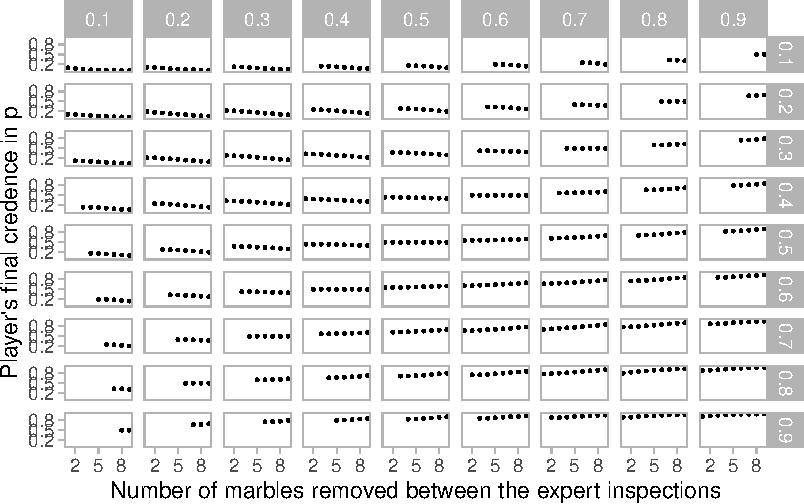
\includegraphics[keepaspectratio]{mixing-experts_files/figure-pdf/fig-conexp-1.pdf}}

}

\caption{\label{fig-conexp}The result of merging two somewhat connected
opinions.}

\end{figure}%

Here is how to read the graph in Figure~\ref{fig-conexp}. Each row
corresponds to a particular credence announced by Ivy; the credence is
shown on the right. Each column corresponds to a particular credence
announced by Zack; that credence is shown on the top. The x-axis of the
individual graphs shows the value for \emph{m}, the number of marbles
removed. And the y-axis shows Player's final credence in \emph{p}. There
are more dots on some graphs than others because some combinations of
Ivy credence, Zack credence and \emph{m} are impossible. The announced
credences can't, by the rules of the game, differ by more than
0.1\emph{m}.

One notable feature of that graph is that as \emph{m} gets larger, the
final credence tends to move away from 0.5; it tends to get more
opinionated. Another notable feature, though probably not one you can
see in this resolution, is that this move towards greater opinionation
happens in a surprisingly linear fashion. To a first approximation,
Player's credence moves away from 0.5 roughly the same amount for each
addition to \emph{m}, at least holding \emph{y} and \emph{z} fixed.

It's not perfectly linear, but it's much closer than I would have
guessed looking at how really quite non-linear the inputs are.
Figure~\ref{fig-cap-bottom-right} shows the result of zooming in on a
part of the graph to see this more vividly.

\begin{figure}

\centering{

\pandocbounded{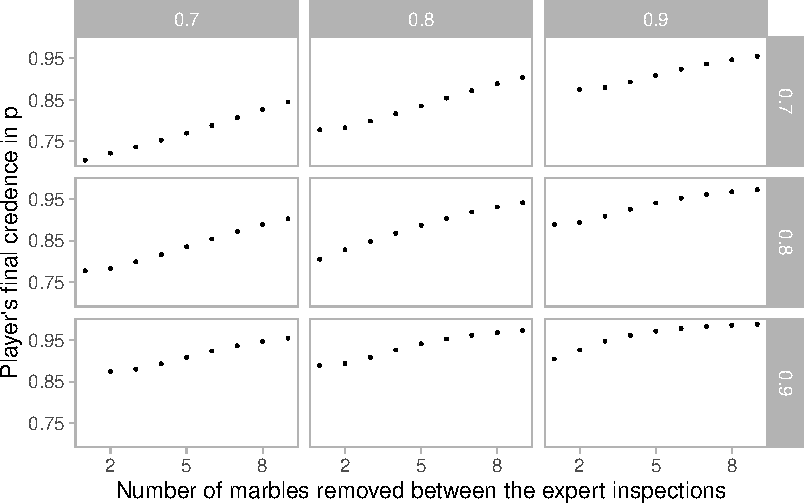
\includegraphics[keepaspectratio]{mixing-experts_files/figure-pdf/fig-cap-bottom-right-1.pdf}}

}

\caption{\label{fig-cap-bottom-right}The bottom right corner of
Figure~\ref{fig-conexp}}

\end{figure}%

The curve in the bottom right panel of Figure~\ref{fig-cap-bottom-right}
is not really linear; it definitely curves downwards. But as you move
your eye upwards and leftwards in the table, the curves look much much
straighter. The panel where they both announce 0.7 is really remarkably
straight. If we focus on the middle of Figure~\ref{fig-conexp}, this is
even more striking. (I've left off the cases where Zack announces a
credence under 0.5 because those graphs are just mirror images of graphs
already shown.)

\begin{figure}

\centering{

\pandocbounded{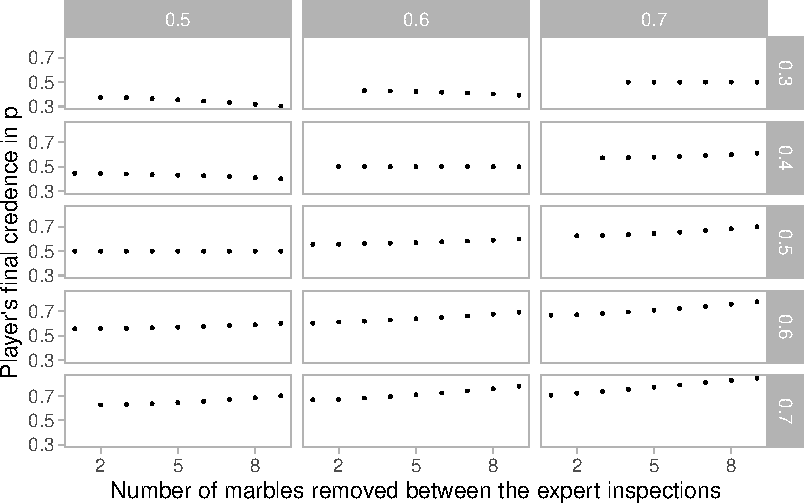
\includegraphics[keepaspectratio]{mixing-experts_files/figure-pdf/fig-cap-middle-1.pdf}}

}

\caption{\label{fig-cap-middle}A detail of the middle of
Figure~\ref{fig-conexp}}

\end{figure}%

Why does this matter? Because pooling functions are easy to use, and the
supra-Bayesian needs something to match that ease of use. It's a cliche
that for every problem there is a solution that is simple, intuitive,
and wrong. And the version of the pooling approach that uses linear
averages is very simple, very intuitive, and very wrong. The version
that uses geometric averages strikes most people as less simple and
intuitive (or maybe I'm just bad at explaining it), but it is less
wrong. But still, sometimes simple, intuitive and wrong is exactly what
you need! Computation is hard, life is short, precision is overrated.
Why not just average if you are just looking to get something roughly
right?

The supra-Bayesian can exploit the more-or-less linearity of the graphs
above graphs to come up with an approximation to these ideal Bayesian
credence. And the approximation isn't that much harder to calculate than
the geometric average. Intuitively, it works like this. If the experts
have exactly the same evidence, we take the geometric average of their
opinions.\footnote{We are working with cases so far where there is a
  unique rational credence for each evidence, so if they have the same
  evidence they have the same credence, and which kind of averaging we
  use is redundant. What matters about the geometric average is how it
  enters into mixtures, as we're about to see.} If the experts' evidence
is conditionally independent, we use the formula from Easwaran et al.
(\citeproc{ref-EaswaranEtAl2016}{2016}) that I rederived in the last
section. In between, we just need a guess \emph{k} about what proportion
of the evidence they share, and what is independent. And we use that
guess to come up with an average of those two things, the geometric
average and the formula for conditionally independent evidence. So our
estimation of the new credence is this, where \emph{y} and \emph{z} are
the announced credences, and \emph{k} is the measure of independence of
the evidence.

\[
(1-k)\frac{\sqrt{yz}}{\sqrt{yz} + \sqrt{(1-y)(1-z)}} + k\frac{yz}{yz + (1-y)(1-z)}
\]

Let's check visually how this does against the exact calculations. In
the graphs that follow, starting with
Figure~\ref{fig-twoprob-bottom-right}, I'll use circles for the ideally
calculated posterior credences, and triangles for the estimates made
using this formula.

\begin{figure}

\centering{

\pandocbounded{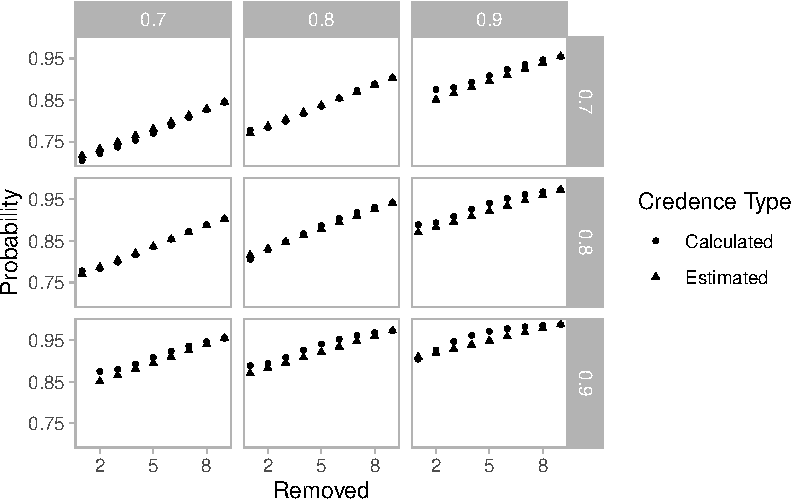
\includegraphics[keepaspectratio]{mixing-experts_files/figure-pdf/fig-twoprob-bottom-right-1.pdf}}

}

\caption{\label{fig-twoprob-bottom-right}A detail from
Figure~\ref{fig-conexp} with estimated probabilities shown.}

\end{figure}%

That looks pretty good. There is a tiny bit of separation in the bottom
right panel of Figure~\ref{fig-twoprob-bottom-right}, but otherwise the
estimate tracks the calculated credences pretty closely.
Figure~\ref{fig-twoprob-middle} shows the middle of the graph.

\begin{figure}

\centering{

\pandocbounded{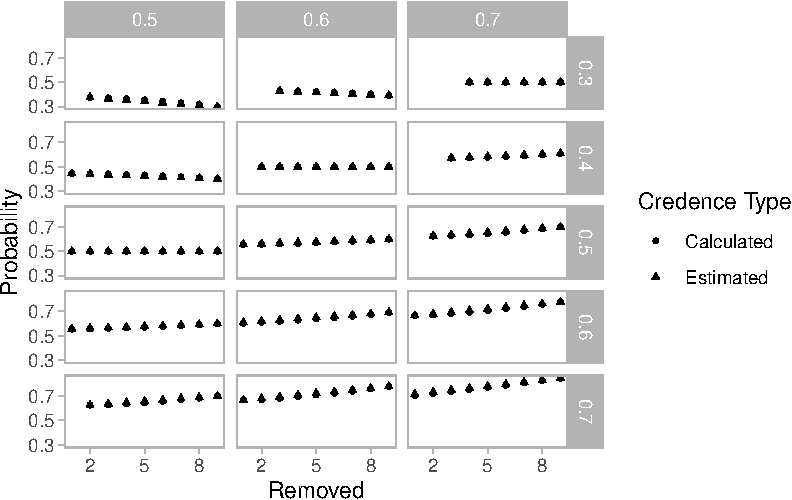
\includegraphics[keepaspectratio]{mixing-experts_files/figure-pdf/fig-twoprob-middle-1.pdf}}

}

\caption{\label{fig-twoprob-middle}The middle of Figure~\ref{fig-conexp}
with estimated probabilities shown.}

\end{figure}%

And all through Figure~\ref{fig-twoprob-middle} the dots are
overlapping. That's close enough. So at least in this special case, the
supra-Bayesian can produce an estimate that is very close to the ideally
calculated credence. So we don't need to resort to pooling even as an
approximation device.

But the simplifications here are dire. Here are six ways we might want
to generalise the model.

\begin{enumerate}
\def\labelenumi{\arabic{enumi}.}
\tightlist
\item
  Have the prior probabilities of \emph{p} and ¬\emph{p} vary.
\item
  Have more colors for the marbles, and have each expert announce
  credences over all the colors.
\item
  Have the person doing the merger be uncertain about \emph{k}.
\item
  Have the experts sample the jars they are given, not inspect them
  fully.
\item
  Have more than two experts.
\item
  Allow that some experts are more informed than others.
\end{enumerate}

The first two points are not that hard. I could produce a string of
graphs for different priors over the colors, or for more colors, and the
typical story is not that different to what we've seen so far. It just
gets messy because we have more degrees of freedom than is consistent
with a concise graphical display.

The next two points are harder. It's not that they are harder to come up
with the ideal value. For any prior over \emph{k}, or sampling technique
that's available to the expert, it's pretty easy to write code to come
up with the optimal calculated credences. It's rather that the number of
degrees of freedom are so great that it gets a little harder to eyeball
how good any given approximation is. The big point is that the posterior
distribution of \emph{k} will usually be different to the prior. In
extreme cases, the announced expert credences might rule out some
hypotheses about \emph{k}. So it won't just be a matter of calculating
the values of the above formula for each value of \emph{k}, and
averaging them out using the prior probabilities of \emph{k}. There is a
lot of possible future research here.

Having more than two experts raises both computational questions, like
what we've just discussed, and conceptual questions. The number of
variables we need to specify to say how connected the experts are
roughly doubles every time one ads an expert. But the point is not just
that the computations of the ideal supra-Bayesian credence require an
exponentially increasing number of inputs as the number of experts
rises. It's that even thinking about how to approximate this ideal
calculation, we need a good way to conceptualise this space whose
dimensionality rises exponentially with the number of experts in a way
that lets us even think about what a good approximation would look like.
I don't have an answer to this; it feels like a question for future
research.

What I will try to make some headway on instead is the last question,
what happens if we do not assume the experts are just as well informed
as each other.

\section{Case Three: Differentially Informed
Experts}\label{case-three-differentially-informed-experts}

In our last case, one expert is better informed than the other. Carmen
first fills the jar with the marked marble and 19 randomly chosen
unmarked marbles. She flips a coin to decide which expert to show this
jar to. They inspect the jar, and record their credence in \emph{p} to
the nearest 0.1. (We'll come back very soon to why this is rounded.)
Carmen then removes 10 unmarked marbles from the jar, chosen at random,
and then shows it to the other expert. They inspect it, and come up with
a new credence in \emph{p}. Then both these recorded numbers are
reported to Player, without any indication about who saw the larger jar
and who saw the smaller one.

There is a weird thing in this setup in that one of the experts reports
something other than their precise credence. The reason I set up the
example this way is to make it impossible for the recipient of the
expert opinion to infer who saw the smaller jar. If they both reported
their actual credence, it would be possible for the recipient to be told
one of them has credence 0.75 in \emph{p} and the other has credence
0.6. And then it would be obvious that the hearer should have credence
0.6 in \emph{p}, since that's the credence of the more informed person.
So I made the first person round to the nearest 0.1 to make it harder to
make such inferences.

Given all that setup we can work out what Player's credence in \emph{p}
should be given the two announcements, and I've shown the values in
Table~\ref{tbl-diffk}. (I'm rounding to three decimal places to save
space.I'm leaving off the cases where one or other party announces an
extremal credence - the hearer agrees with those credences, at least to
three decimal places. And the `NA' values are where it is impossible
given the setup for those to be the announced values.)

\begin{longtable}[]{@{}
  >{\raggedleft\arraybackslash}p{(\linewidth - 18\tabcolsep) * \real{0.1429}}
  >{\raggedleft\arraybackslash}p{(\linewidth - 18\tabcolsep) * \real{0.0952}}
  >{\raggedleft\arraybackslash}p{(\linewidth - 18\tabcolsep) * \real{0.0952}}
  >{\raggedleft\arraybackslash}p{(\linewidth - 18\tabcolsep) * \real{0.0952}}
  >{\raggedleft\arraybackslash}p{(\linewidth - 18\tabcolsep) * \real{0.0952}}
  >{\raggedleft\arraybackslash}p{(\linewidth - 18\tabcolsep) * \real{0.0952}}
  >{\raggedleft\arraybackslash}p{(\linewidth - 18\tabcolsep) * \real{0.0952}}
  >{\raggedleft\arraybackslash}p{(\linewidth - 18\tabcolsep) * \real{0.0952}}
  >{\raggedleft\arraybackslash}p{(\linewidth - 18\tabcolsep) * \real{0.0952}}
  >{\raggedleft\arraybackslash}p{(\linewidth - 18\tabcolsep) * \real{0.0952}}@{}}

\caption{\label{tbl-diffk}The posterior probability after hearing two
differentially informed experts.}

\tabularnewline

\toprule\noalign{}
\begin{minipage}[b]{\linewidth}\raggedleft
Ivy/Zack
\end{minipage} & \begin{minipage}[b]{\linewidth}\raggedleft
0.1
\end{minipage} & \begin{minipage}[b]{\linewidth}\raggedleft
0.2
\end{minipage} & \begin{minipage}[b]{\linewidth}\raggedleft
0.3
\end{minipage} & \begin{minipage}[b]{\linewidth}\raggedleft
0.4
\end{minipage} & \begin{minipage}[b]{\linewidth}\raggedleft
0.5
\end{minipage} & \begin{minipage}[b]{\linewidth}\raggedleft
0.6
\end{minipage} & \begin{minipage}[b]{\linewidth}\raggedleft
0.7
\end{minipage} & \begin{minipage}[b]{\linewidth}\raggedleft
0.8
\end{minipage} & \begin{minipage}[b]{\linewidth}\raggedleft
0.9
\end{minipage} \\
\midrule\noalign{}
\endhead
\bottomrule\noalign{}
\endlastfoot
0.1 & 0.100 & 0.103 & 0.100 & 0.100 & 0.100 & 0.100 & NA & NA & NA \\
0.2 & 0.103 & 0.200 & 0.208 & 0.203 & 0.202 & 0.200 & NA & NA & NA \\
0.3 & 0.100 & 0.208 & 0.300 & 0.320 & 0.325 & 0.348 & 0.500 & NA & NA \\
0.4 & 0.100 & 0.203 & 0.320 & 0.400 & 0.439 & 0.500 & 0.652 & 0.800 &
0.900 \\
0.5 & 0.100 & 0.202 & 0.325 & 0.439 & 0.500 & 0.561 & 0.675 & 0.798 &
0.900 \\
0.6 & 0.100 & 0.200 & 0.348 & 0.500 & 0.561 & 0.600 & 0.680 & 0.797 &
0.900 \\
0.7 & NA & NA & 0.500 & 0.652 & 0.675 & 0.680 & 0.700 & 0.792 & 0.900 \\
0.8 & NA & NA & NA & 0.800 & 0.798 & 0.797 & 0.792 & 0.800 & 0.897 \\
0.9 & NA & NA & NA & 0.900 & 0.900 & 0.900 & 0.900 & 0.897 & 0.900 \\

\end{longtable}

And a striking thing about Table~\ref{tbl-diffk} is how close it comes
to verifying a strong form of what Levinstein
(\citeproc{ref-Levinstein2015}{2015}) calls Thrasymachus' Principle. The
hearer defers to the expert with the strongest view, i.e., the view
that's furthest from the prior. In contemporary terms, the hearer
listens to the expert with the hottest take. It isn't an unvarnished
form of that. When one says 0.5 and the other says 0.6 you end up with
0.561, not 0.6. But that's in large part because there's a good chance
that the person who said 0.6 was merely rounding up as the result of a
coin flip. In general, the rule in this case is find the expert credence
that is furthest from the prior, and adopt it.

There is a reason that a case like this should follow Thrasymachus'
Principle. If the experts are rational, hotter takes should correspond
to stronger evidence. And while it isn't impossible for the person with
more evidence to have in a sense weaker evidence, the extra evidence may
be full of defeaters for the first obtained evidence, it is pretty
unlikely. In general, if someone is worthy of deference, and they have a
strong view, they have strong evidence. If someone else has a weaker
view, i.e., a view closer to the prior, the best explanation is that
they simply don't have the evidence that the person with stronger view
does.

So again, we shouldn't pool the opinions in any interesting sense. The
table shows the optimal response by supra-Bayesian lights. And the
simple approximation is, ``When one expert has clearly stronger views,
listen to them. Otherwise take the geometric mean.''

\section{Summary}\label{summary}

Let's take stock of what's been covered so far.

\begin{itemize}
\tightlist
\item
  I've argued against all three uses of pooling answers to the question
  of how to merge expert opinions. Sometimes the pooling answer is
  clearly wrong, often it won't be a good constraint on priors, and
  there are better ways to approximate the correct supra-Bayesian
  answer.
\item
  I've connected supra-Bayesianism to some familiar positions in
  epistemology, the view on testimony in Jackson
  (\citeproc{ref-Jackson1987}{1987}) and the view on disagreement in
  Lackey (\citeproc{ref-Lackey2010-LACWSW}{2010}).
\item
  I've shown that if you take that approach, that conditionalising on
  someone else's credence is just conditionalising on the fact that they
  have evidence that rationalises such a credence by their lights, then
  the principle Easwaran et al. (\citeproc{ref-EaswaranEtAl2016}{2016})
  recommend for updating on the credences of others follows directly
  from the assumptions that each expert is independently worthy of
  deference, and the evidence the experts have is conditionally
  independent.
\item
  I've developed a toy example that lets us think about cases where the
  hearer doesn't know which parts of the evidence are in common, but
  does know how much is in common.
\item
  And I've shown that in that case, the correct supra-Bayesian answer is
  nicely approximated by a linear average of two familiar formulas.
\item
  I developed a toy example that lets us think about the case where one
  expert is known to be more informed, but we aren't sure which it is.
\item
  And in that case I showed that what Levinstein
  (\citeproc{ref-Levinstein2015}{2015}) calls Thrasymachus' Principle is
  approximately right; we should defer to the `stronger', i.e., more
  opinionated, expert.
\end{itemize}

At the end of section 2 I mentioned six ways in which we might make the
model even more general. This is very much not meant to be the last
word. But I suspect these kinds of examples can be used to provide
useful approximations, or guides, to real life situations where we know
something about the relationship between the experts. The general lesson
is that by looking at toy cases, we can provide practical advice for how
to emulate, or at least approximate, the supra-Bayesian approach for
merging expert opinion. And this advice will be better than the advice
that anyone who ignores the relationship between the experts can offer.

But there is one last kind of relationship between experts that I
haven't made any progress on modelling, and it is a big one. What should
we say about cases where the experts know each others credences? This is
an old and, to my mind, open question. For reasons that trace back to
Aumann (\citeproc{ref-Aumann1976}{1976}), in anything like the kind of
model I've used here, if the experts know each other's credences, they
have to agree. And someone who knows both credences should agree with
them. But the real world obviously contains experts who do agree to
disagree. What to say about those cases is the biggest open questions
around here, and I'm not sure whether this approach can help. Gallow
(\citeproc{ref-Gallow2018}{2018}) ends his paper by raising doubts about
whether it is rational to be disposed to defer to two different experts.
I'm not worried about that in general; I've described three very
different kinds of cases where it is rational. But I suspect one could
not be rationally disposed to defer to two experts who one knows are
themselves disposed to agree to disagree. That, however, is a story for
another paper. This paper has described a number of cases where the
hearer knows something the experts doesn't know: namely what other
experts think. And it has described both precise and approximate answers
for what to do in those interesting cases.

\subsection*{References}\label{references}
\addcontentsline{toc}{subsection}{References}

\phantomsection\label{refs}
\begin{CSLReferences}{1}{0}
\bibitem[\citeproctext]{ref-Aumann1976}
Aumann, Robert J. 1976. {``Agreeing to Disagree.''} \emph{The Annals of
Statistics} 4 (6): 1236--39. doi:
\href{https://doi.org/10.1214/aos/1176343654}{10.1214/aos/1176343654}.

\bibitem[\citeproctext]{ref-BaccelliStewart2021}
Baccelli, Jean, and Rush T. Stewart. 2021. {``Support for Geometric
Pooling.''} \emph{Review of Symbolic Logic} forthcoming. doi:
\href{https://doi.org/doi:10.1017/S1755020320000416}{doi:10.1017/S1755020320000416}.

\bibitem[\citeproctext]{ref-Bradley2017}
Bradley, Richard. 2017. {``Learning from Others: Conditioning Versus
Averaging.''} \emph{Theory and Decision} 85 (1): 5--20. doi:
\href{https://doi.org/10.1007/s11238-017-9615-y}{10.1007/s11238-017-9615-y}.

\bibitem[\citeproctext]{ref-EaswaranEtAl2016}
Easwaran, Kenny, Luke Fenton-Glynn, Christopher Hitchcock, and Joel D.
Velasco. 2016. {``Updating on the Credences of Others: Disagreement,
Agreement, and Synergy.''} \emph{Philosophers' Imprint} 16 (11): 1--39.

\bibitem[\citeproctext]{ref-Elga2007}
Elga, Adam. 2007. {``Reflection and Disagreement.''} \emph{No{û}s} 41
(3): 478--502. doi:
\href{https://doi.org/10.1111/j.1468-0068.2007.00656.x}{10.1111/j.1468-0068.2007.00656.x}.

\bibitem[\citeproctext]{ref-Gallow2018}
Gallow, J. Dmitri. 2018. {``No One Can Serve Two Epistemic Masters.''}
\emph{Philosophical Studies} 175 (10): 2389--98. doi:
\href{https://doi.org/10.1007/s11098-017-0964-8}{10.1007/s11098-017-0964-8}.

\bibitem[\citeproctext]{ref-Jackson1987}
Jackson, Frank. 1987. \emph{Conditionals}. Blackwell: Oxford.

\bibitem[\citeproctext]{ref-Lackey2010-LACWSW}
Lackey, Jennifer. 2010. {``What Should We Do When We Disagree.''}
\emph{Oxford Studies in Epistemology} 3: 274--93.

\bibitem[\citeproctext]{ref-Levinstein2015}
Levinstein, Benjamin Anders. 2015. {``With All Due Respect: The
Macro-Epistemology of Disagreement.''} \emph{Philosophers' Imprint} 15
(13): 1--20.

\bibitem[\citeproctext]{ref-RussellEtAl2015}
Russell, Jeffrey Sanford, John Hawthorne, and Lara Buchak. 2015.
{``Groupthink.''} \emph{Philosophical Studies} 172 (5): 1287--1309. doi:
\href{https://doi.org/10.1007/s11098-014-0350-8}{10.1007/s11098-014-0350-8}.

\end{CSLReferences}



\noindent Unpublished. Posted online in 2021.


\end{document}
